%----------------------------------------------------------------------------
\chapter{CARLA Simulator}
\label{chap:carlasim}
%----------------------------------------------------------------------------

CARLA's mission is to create a simulator that can simulate sufficient-enough
real-world traffic scenarios so that it is more accessible for researchers like
myself to research, develop and test computer vision algorithms for
self-driving car. 

CARLA~\cite{Dosovitskiy17} is an open-source simulator for autonomous driving
research. It is written in C++ and provides an accessible Python API to
control the simulaton execution. It has been developed from the ground
up to support development, training, and validation of autonomous driving
systems. In addition to open-source code and protocols, CARLA provides open
digital assets (urban layouts, buildings, vehicles) that were created for this
purpose and can be used freely. The simulation platform supports flexible
specification of sensor suites, environmental conditions, full control of all
static and dynamic actors, maps generation and much more. It is developed by the
Barcelonian university UAB's computer vision CVC Lab and supported by companies
such as Intel, Toyota, GM and others. The repository for the project is at
\url{https://github.com/carla-simulator}

It provides scalability via a server multi-client architecture: multiple clients
in the same or in different nodes can control different actors. Carla exposes a
powerful API that allows users to control all aspects related to the simulation,
including traffic generation, pedestrian behaviors, weathers, sensors, and much
more. Users can configure diverse sensor suites including LIDARs, multiple
cameras, depth sensors and GPS among others. Users can easily create their own
maps following the OpenDrive standard via tools like RoadRunner. Furthermore it
provides integration with ROS\footnote{Robot Operating System (ROS)
\url{https://www.ros.org/}} via their ROS-bridge

I used CARLA 9.8.0 in the project that was the latest at the time (2020 March
09). Carla has a primary support for Linux so I could run it easly on Ubuntu. It
requires a decent GPU otherwise the simulation is going to be slow.

It's important to mind the coordinate system used in Carla, because later when
we will extract data the axes must be mapped to the correct data points. Since
Carla is built with Unreal Engine \footnote{Unreal Engine
\url{https://www.unrealengine.com/}} it uses the coordinate system as in
\autoref{fig:carlacoords}: X coordinate is to the front of the ego actor, Y is to the
right of ego and Z is to the top.

\begin{figure}[!ht]
  \centering
  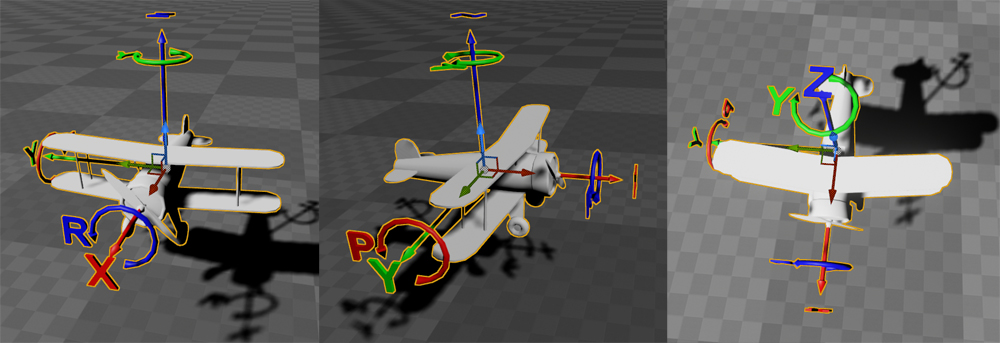
\includegraphics[width=150mm, keepaspectratio]{figures/carlacoords.jpg}
  \caption{Carla coordinate system}
  \label{fig:carlacoords}
\end{figure}


\section{Is a simulation enough?}
I believe the future of self-driving car research and development is in part
with simulations and in part with real-world training as well. To develop a
self-driving AI from ground up it is certainly advisable to first develop and
test the algorithms in a simulation. 

In order to create simulations that are rich and different Carla provides a
large variety of actors and maps. The traffic manager can also be parametrized
to control how pedestrians and vehicles move: their speed, minimum distance, and
even "aggressivity" towards each other, which means how willing are
they to collide instead of waiting until the actor in front moves away. This is
actually useful as it helps unlock possible traffic deadlocks. The latest
CARLA provides 8 maps but in newer versions they will be adding new maps. You
can see a screenshot of each rendering in the 6 maps I used in
\autoref{fig:maps}.

\begin{figure}[!ht]
  \centering
  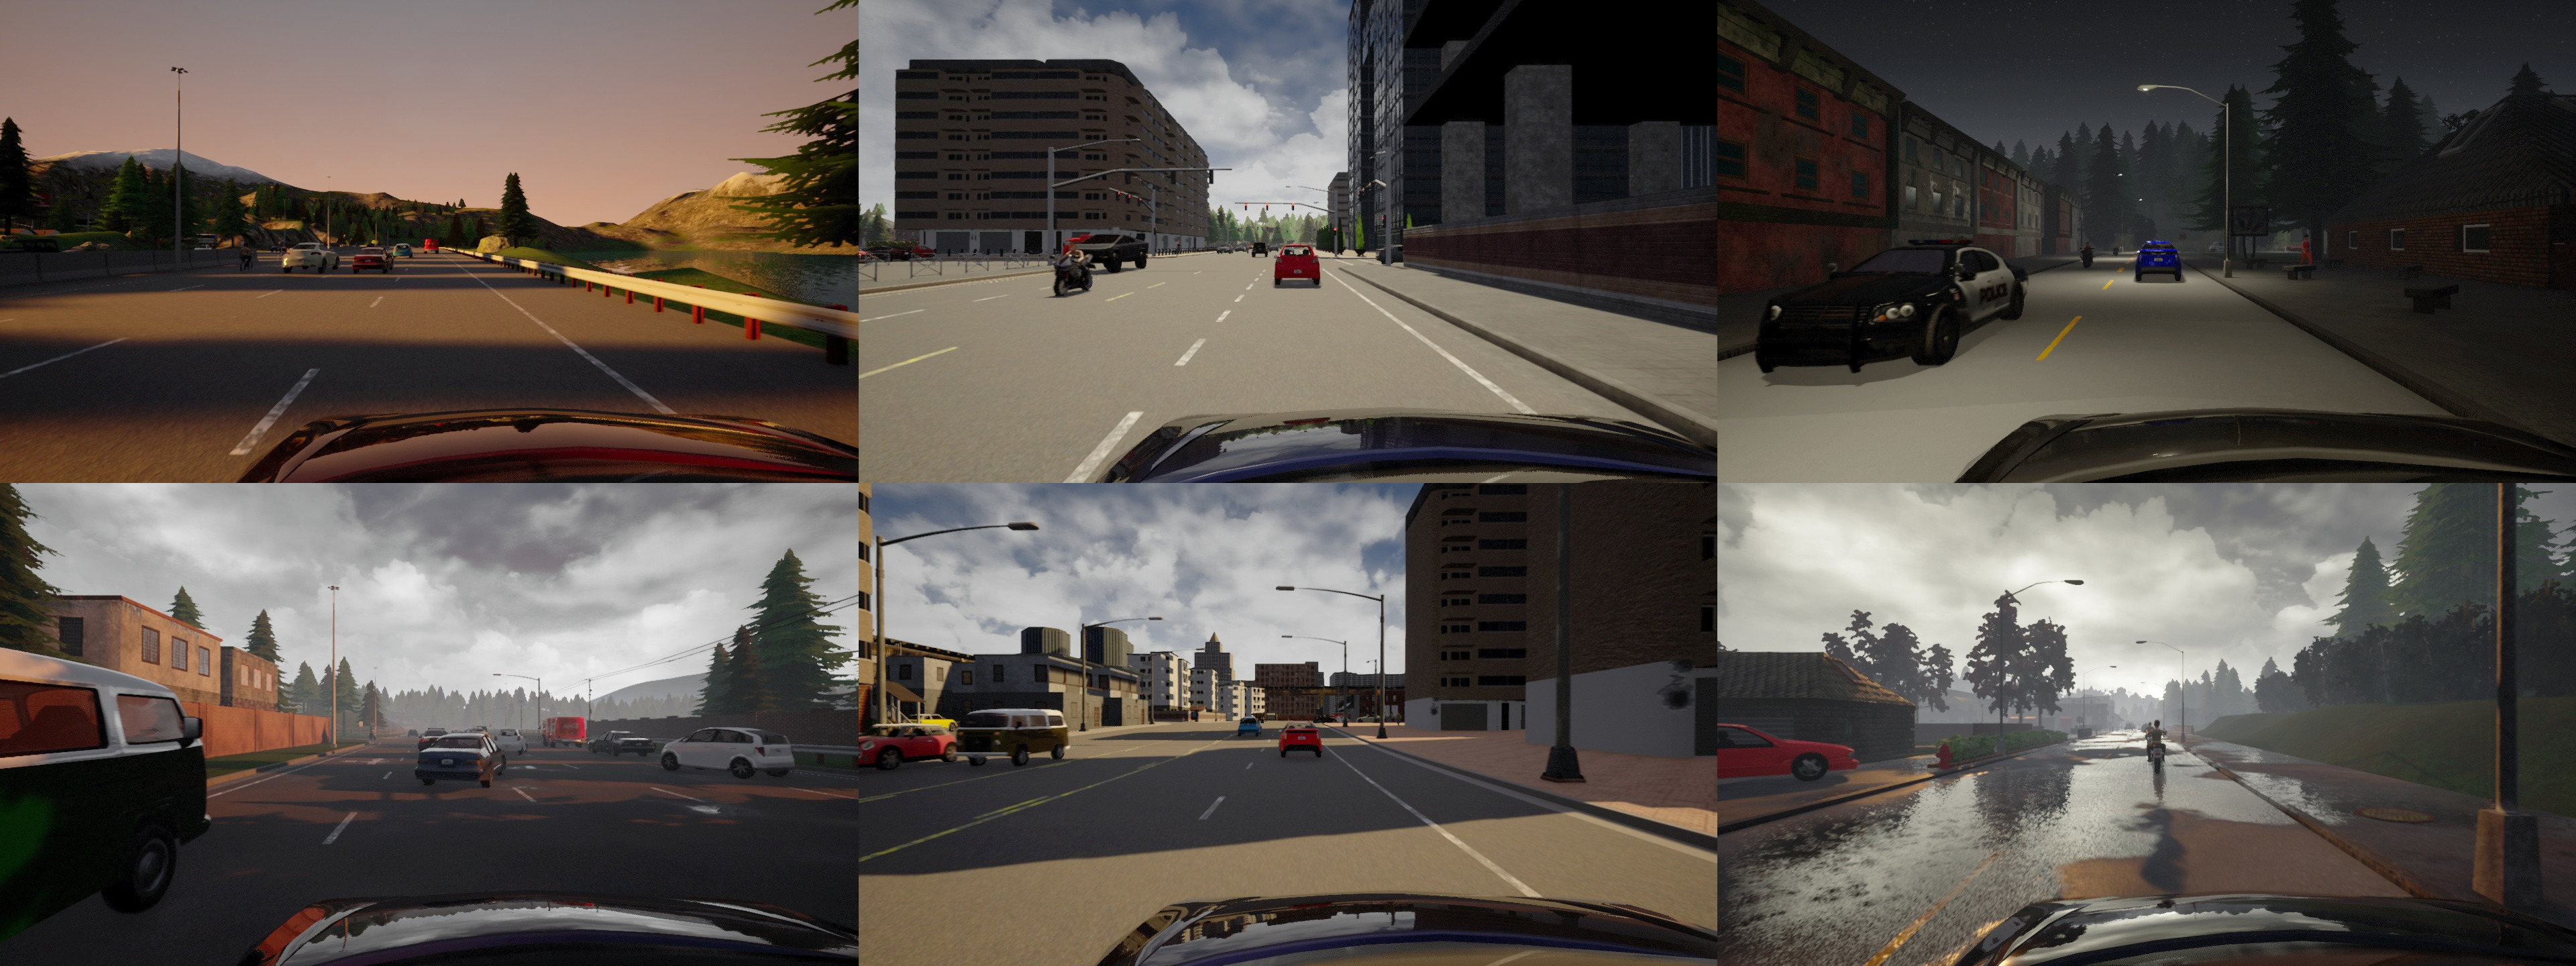
\includegraphics[width=150mm, keepaspectratio]{figures/maps.jpg}
  \caption{Variety of maps in Carla}
  \label{fig:maps}
\end{figure}

A simulation obviously can't return the variety and exact nature of scenarios
that happen in \emph{nature}. However I believe they are sufficient for testing
an entry-level self-driving system and that with the use of simulations a
company can lower the costs of development. The rise of simulators itself shows
there is a need for the market.

\section{CARLA Simulation sensors}

The Carla simulator's API support a wide range of sensors: RGB Cameras, LiDAR,
Radar, GPS, gyroscope, accelerometer, compass and more. These are easy to
use, If you are interested I recommend reading the sensors reference in their
documentation \footnote{CARLA sensors reference
\url{https://carla.readthedocs.io/en/latest/ref_sensors/}}

Carla also provides miscellaneous sensors that help collecting ground-truth data
for deep learning applications. This includes semantic segmentation camera,
depthmap camera and other simple ones such as collision detector as seen in \autoref{fig:carlaseg}.

\begin{figure}[!ht]
  \centering
  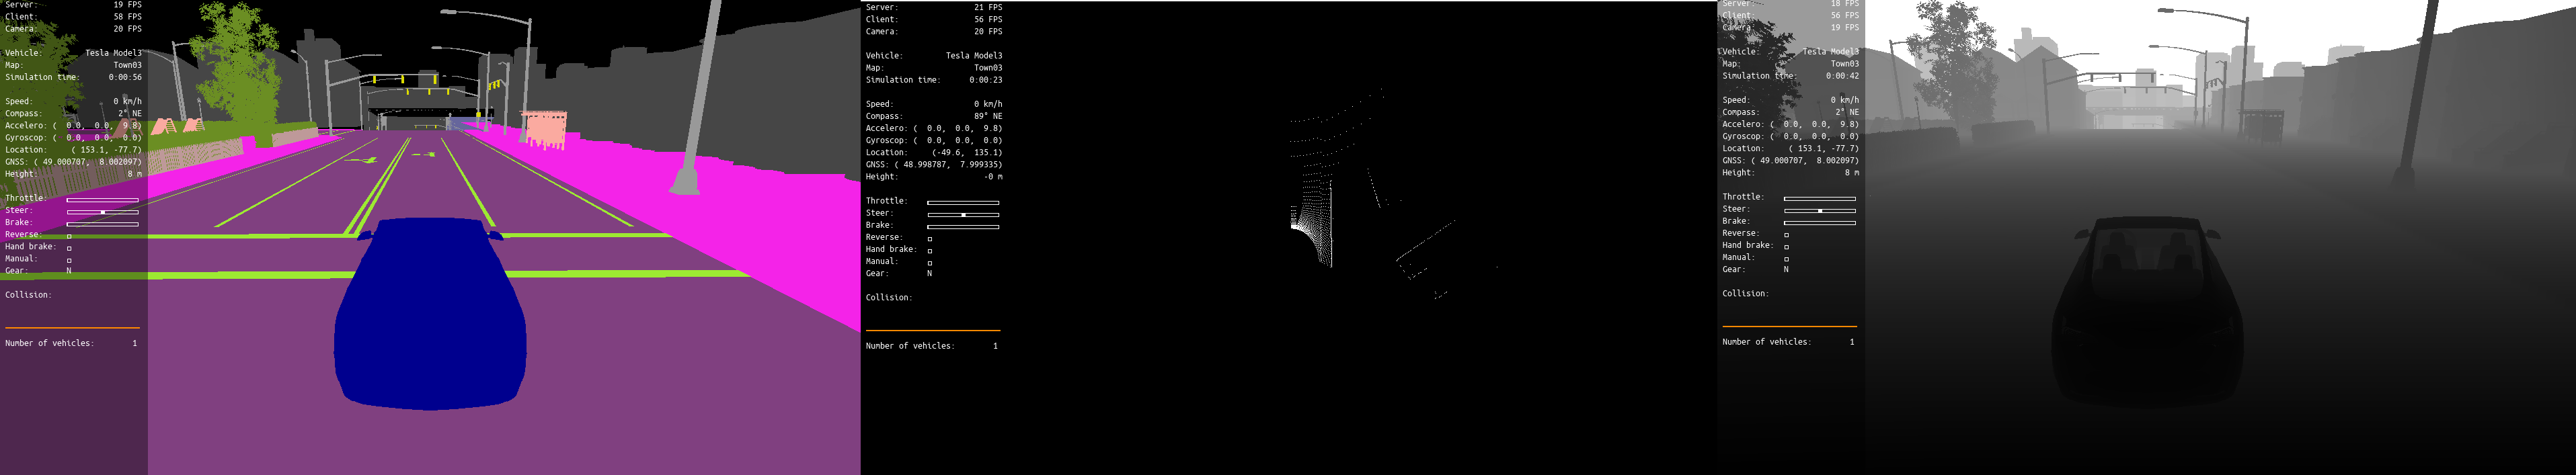
\includegraphics[width=150mm, keepaspectratio]{figures/carlaseg.png}
  \caption{Different sensors and cameras in Carla (semantic segmentation, lidar, depthmap)}
  \label{fig:carlaseg}
\end{figure}

\subsection{Other simulators}

There are a couple of other dedicated projects for simulators. There is
Deepdrive from Voyage auto\footnote{Deepdrive Voyage
\url{https://deepdrive.voyage.auto/}}, an American AD supplier, NVIDIA has a
project going on called Drive Constellation\footnote{NVIDIA Drive Constellation
\url{https://developer.nvidia.com/drive/drive-constellation}} which is said to
be advanced but is not opensource. Nvidia provides Harware In the Loop
simulation for Drive Constellation which is an even more advanced simulation
infrastructure that allows for testing the systems real-timeness. There is
another project called RFPro\footnote{RFPro \url{http://www.rfpro.com/}}.
However these are either not opensource or not mature enough. CARLA
Simulator~\cite{Dosovitskiy17} was by far the best one
for my case.